
%(BEGIN_QUESTION)
% Copyright 2014, Tony R. Kuphaldt, released under the Creative Commons Attribution License (v 1.0)
% This means you may do almost anything with this work of mine, so long as you give me proper credit

In this graph of two AC voltages, which one is {\it leading} and which one is {\it lagging}?

$$\includegraphics[width=15.5cm]{i00839x01.eps}$$

If the 4-volt (peak) sine wave is denoted in phasor notation as $4 \hbox{ V} \angle \> 0^o$, how should the 3-volt (peak) waveform be denoted?  Express your answer in both polar and rectangular forms.

\vskip 5pt

If the 4-volt (peak) sine wave is denoted in phasor notation as $4 \hbox{ V} \angle \> 90^o$, how should the 3-volt (peak) waveform be denoted?  Express your answer in both polar and rectangular forms.

\underbar{file i00839}
%(END_QUESTION)





%(BEGIN_ANSWER)

The 4-volt (peak) waveform {\it leads} the 3-volt (peak) waveform.  Conversely, the 3-volt waveform {\it lags} behind the 4-volt waveform.

\vskip 5pt

If the 4-volt waveform is denoted as 4 V $\angle$ 0$^o$, then the 3-volt waveform should be denoted as 3 V $\angle$ $-90^o$, or $0 - j3$ V.

\vskip 5pt

If the 4-volt waveform is denoted as 4 V $\angle$ 90$^o$ ($0 + j4$ V in rectangular form), then the 3-volt waveform should be denoted as 3 V $\angle$ 0$^o$, or $3 + j0$ V.


%(END_ANSWER)





%(BEGIN_NOTES)


%INDEX% Electricity review: phase shift measurement (dual-trace oscilloscope)

%(END_NOTES)

